\documentclass[11pt]{article}
\usepackage[utf8]{inputenc}
\usepackage[T1]{fontenc}
\usepackage{amsmath}
\usepackage{multicol}
\usepackage{geometry}
\usepackage{tikz}
\usetikzlibrary{shapes.geometric, arrows.meta, calc}
\usepackage{enumitem}
\usepackage{xcolor}
\usepackage{titlesec}
\usepackage{mdframed} % substituto mais leve para tcolorbox

% Configurações de layout
\geometry{a4paper, left=1cm, right=1cm, top=0.5cm, bottom=1.2cm}
\setlength{\columnseprule}{0.4pt}
\setlength{\baselineskip}{1.0\baselineskip}

% Cores personalizadas
\definecolor{titleblue}{RGB}{0,80,150}
\definecolor{sectionred}{RGB}{180,0,0}
\definecolor{darkgreen}{RGB}{0,100,0}
\definecolor{examplebg}{RGB}{240,248,255}

% Formatação de títulos
\titleformat{\section}{\normalfont\Large\bfseries\color{titleblue}}{\thesection}{1em}{}
\titleformat{\subsection}{\normalfont\large\bfseries\color{sectionred}}{\thesubsection}{1em}{}
\titleformat{\subsubsection}{\normalfont\normalsize\bfseries\color{darkgreen}}{\thesubsubsection}{1em}{}

\title{\textcolor{titleblue}{Análise Combinatória - Aula Completa}}
\author{Professor: Jefferson}
\date{}

\begin{document}

\maketitle
\vspace{-1cm}

\begin{center}
\large{Nome: \underline{\hspace{8cm}} \quad Turma: \underline{\hspace{3cm}}}
\end{center}

\begin{multicols}{2}

\section*{Introdução}
A Análise Combinatória estuda \textbf{como contar} possibilidades sem precisar enumerar todas elas. É essencial para probabilidade e situações do cotidiano.

\section*{1. Princípio Fundamental da Contagem (PFC)}

\subsection*{O que é?}
É a \textbf{regra do "e"} para eventos consecutivos e independentes.

\begin{mdframed}[backgroundcolor=examplebg, linecolor=blue!50!black]
\textbf{Exemplo Prático}

\underline{Situação}: Você tem:
\begin{itemize}
\item 3 camisetas: Azul (A), Vermelha (V), Verde (Vd)
\item 2 calças: Jeans (J), Preta (P)
\end{itemize}
Quantas combinações diferentes você pode fazer?

\underline{Solução}:
\begin{enumerate}
\item Para cada camiseta (3 opções), você pode escolher qualquer calça (2 opções)
\item Total = 3 (camisetas) × 2 (calças) = 6 combinações
\end{enumerate}

\begin{center}
\begin{tabular}{|c|c|}
\hline
Combinação & Peças \\
\hline
1 & A + J \\
2 & A + P \\
3 & V + J \\
4 & V + P \\
5 & Vd + J \\
6 & Vd + P \\
\hline
\end{tabular}
\end{center}
\end{mdframed}

\subsection*{Fórmula Geral}
Se temos:
\begin{itemize}
\item 1ª escolha: m opções
\item 2ª escolha: n opções
\item ...
\item k-ésima escolha: p opções
\end{itemize}

O número total de possibilidades é:

\[ \boxed{m \times n \times \cdots \times p} \]

\section*{2. Permutação}

\subsection*{2.1 Permutação Simples}
Quando \textbf{ordenamos todos} os elementos distintos.

\[ P_n = n! \]
(Onde $n! = n \times (n-1) \times \cdots \times 1$ e $0! = 1$)

\begin{mdframed}[backgroundcolor=examplebg, linecolor=blue!50!black]
\textbf{Exemplo Passo a Passo}

Quantos anagramas tem a palavra "AMOR"?

\underline{Resolução}:
\begin{enumerate}
\item Temos 4 letras distintas: A, M, O, R
\item Para a 1ª posição: 4 opções
\item Para a 2ª posição: 3 opções restantes
\item Para a 3ª posição: 2 opções
\item Para a 4ª posição: 1 opção
\item Total = $4 \times 3 \times 2 \times 1 = 4! = 24$
\end{enumerate}
\end{mdframed}

\subsection*{2.2 Permutação com Repetição}
Quando há elementos repetidos:

\[ P_n^{n_1,n_2,\dots,n_k} = \frac{n!}{n_1! \times n_2! \times \cdots \times n_k!} \]

\begin{mdframed}[backgroundcolor=examplebg, linecolor=blue!50!black]
\textbf{Exemplo Detalhado}

Quantos anagramas tem "BANANA"?

\underline{Passo a Passo}:
\begin{enumerate}
\item Total de letras: 6 (B, A, N, A, N, A)
\item Letras repetidas: 3 A's e 2 N's
\item Cálculo:
\[ \frac{6!}{3! \times 2!} = \frac{720}{6 \times 2} = 60 \]
\end{enumerate}
\end{mdframed}

\section*{3. Arranjo}

\subsection*{Quando usar?}
Quando a \textbf{ordem importa} e \textbf{não usamos todos} os elementos.

\[ A_{n,p} = \frac{n!}{(n-p)!} \]

\begin{mdframed}[backgroundcolor=examplebg, linecolor=blue!50!black]
\textbf{Exemplo Comentado}

Num pódio com 1º, 2º e 3º lugares, com 10 competidores.

\underline{Por que é arranjo?}:
\begin{itemize}
\item A ordem importa (1º ≠ 2º ≠ 3º)
\item Não usamos todos os 10 competidores
\end{itemize}

\underline{Cálculo}:
\[ A_{10,3} = 10 \times 9 \times 8 = 720 \]
\end{mdframed}

\section*{4. Combinação}

\subsection*{Quando usar?}
Quando a \textbf{ordem não importa} e formamos grupos.

\[ C_{n,p} = \binom{n}{p} = \frac{n!}{p!(n-p)!} \]

\subsection*{Princípio do Desprezo de Ordem}
\begin{mdframed}[backgroundcolor=yellow!10, linecolor=yellow!50!black]
\textbf{Entendendo a Diferença}

\underline{Arranjo vs Combinação}:
\begin{itemize}
\item \textbf{Arranjo}: ABC $\neq$ ACB (ordem diferente = resultado diferente)
\item \textbf{Combinação}: ABC $=$ ACB $=$ BAC $= \cdots $ (são o mesmo grupo)
\end{itemize}

\underline{Por que dividimos por p! na combinação?}:
Para eliminar as repetições de ordem. Exemplo para grupo ABC:
\begin{itemize}
\item 3! = 6 permutações (ABC, ACB, BAC, BCA, CAB, CBA)
\item Na combinação, todas contam como 1 único grupo
\end{itemize}
\end{mdframed}

\begin{mdframed}[backgroundcolor=examplebg, linecolor=blue!50!black]
\textbf{Exemplo Visual}

Quantos triângulos formamos com 5 pontos não colineares?

\begin{center}
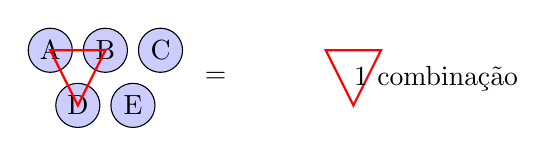
\begin{tikzpicture}[scale=0.7]
    \foreach \x/\y/\t in {0/0/A,1/0/B,2/0/C,0.5/-1/D,1.5/-1/E} {
        \draw[fill=blue!20] (\x,\y) circle (0.4) node {\t};
    }
    \draw[red, thick] (0,0) -- (1,0) -- (0.5,-1) -- cycle;
    \node at (3,-0.5) {=};
    \draw[red, thick] (5,0) -- (5.5,-1) -- (6,0) -- cycle;
    \node at (7,-0.5) {1 combinação};
\end{tikzpicture}
\end{center}

\underline{Solução}:
\[ C_{5,3} = \frac{5!}{3!2!} = 10 \text{ triângulos} \]
\end{mdframed}

\section*{5. Resumo Visual}

\begin{center}
\renewcommand{\arraystretch}{1.8}
\begin{tabular}{|c|c|c|c|}
\hline
\textbf{Conceito} & \textbf{Quando usar?} & \textbf{Fórmula} & \textbf{Exemplo} \\
\hline
PFC & Eventos consecutivos & $m \times n \times p$ & Lanches combinados \\
\hline
Permutação & Ordenar todos & $n!$ & Anagramas \\
\hline
Arranjo & Ordem importa, não usa todos & $\frac{n!}{(n-p)!}$ & Senhas, pódios \\
\hline
Combinação & Ordem não importa & $\frac{n!}{p!(n-p)!}$ & Comissões, grupos \\
\hline
\end{tabular}
\end{center}

\section*{6. Exercícios Resolvidos}

\begin{enumerate}
    \item \underline{Problema}: Um restaurante oferece 5 pratos principais, 3 acompanhamentos e 2 sobremesas. Quantas refeições completas distintas podem ser formadas?
    
    \underline{Solução}:
    \begin{itemize}
    \item Pelo PFC: $5 \times 3 \times 2 = 30$ possibilidades
    \end{itemize}
    
    \item \underline{Problema}: Quantos números de 3 algarismos distintos podemos formar com 1,2,3,4,5?
    
    \underline{Solução}:
    \begin{itemize}
    \item É arranjo (ordem importa e não usa todos): $A_{5,3} = 5 \times 4 \times 3 = 60$
    \end{itemize}
    
    \item \underline{Problema}: Quantas comissões de 3 pessoas podemos formar com 7 alunos?
    
    \underline{Solução}:
    \begin{itemize}
    \item É combinação (ordem não importa): $C_{7,3} = \frac{7!}{3!4!} = 35$
    \end{itemize}
\end{enumerate}

\section*{7. Exercícios Propostos}

\begin{enumerate}
    \item Você tem 4 pares de sapatos e 5 bonés. De quantas maneiras diferentes pode calçar um par de sapatos e usar um boné?
    
    \item Quantos anagramas tem a palavra "ARARA"?
    
    \item Numa classe de 30 alunos, de quantas formas podemos escolher:
    \begin{itemize}
    \item Um presidente e um vice?
    \item Uma dupla para representar a turma?
    \end{itemize}
    
    \item (Desafio) Quantas diagonais tem um polígono de 12 lados?
    \textit{Dica}: Lembre-se que diagonais são segmentos que não são lados do polígono.
\end{enumerate}

\end{multicols}

\end{document}

